\chapter{The \LHC and the \CMS experiment}
\label{chap:detector}

%\chapterquote{There, sir! that is the perfection of vessels!}
%{Jules Verne, 1828--1905}
The purpose of this chapter is to introduce the \CMS experiment and the \LHC \cite{1748-0221-3-08-S08001}. Without both of these apparatus the analyses performed for this thesis would, of course, not have been possible. In \SectionRef{sec:lhc} an overview of the \LHC and the chain of accelerators which feed into it will be given. This will then be followed in \SectionRef{sec:CMSInDetail} by a description of the \CMS experiment focussing on the aspects most relevant to the search for invisibly decaying Higgs bosons.

\section{The \LHC}
\label{sec:lhc}
The \LHC is situated 100m underground in a tunnel formerly built for the LEP accelerator~\cite{lepdesign} at CERN near Geneva, Switzerland. It is a 27km storage ring which accelerates both protons and heavy ions and collides them at the highest centre of mass energies of any collider built to date. The work contained in this thesis uses data from proton-proton collisions. These protons are obtained by taking hydrogen gas and stripping its atoms of their electrons with an electric field. The first accelerator in the \LHC accelerator sequence, Linac 2, then accelerates the protons to 50 \MeV. The protons are then accelerated to 1.4 \GeV~by the next accelerator, the Proton Synchrotron Booster (PSB), which is followed by the Proton Synchrotron (PS) where they reach 25 \GeV. The beam energy is then increased to 450 \GeV~in the Super Proton Synchrotron (SPS). The protons are then injected into the \LHC where, at time of writing, the maximum energy the beams have been accelerated to is 6.5 \TeV, close to the design maximum of 7 \TeV.

When fully filled the \LHC contains two counter-rotating beams which are formed of up to 2808 bunches spaced either 25 or 50 ns apart and each containing $\mathcal{O}(10^{11})$ protons. The two beams are kept travelling in a cirlce by 1232 superconducting dipole magnets and steered to four collision points around the \LHC. Detectors are situated at these collision points to observe the collisions, the main four being: ALICE~\cite{Aamodt:2008zz}, ATLAS~\cite{Aad:1129811}, CMS~\cite{Chatrchyan:2008aa} and LHCb~\cite{Alves:2008zz}. A schematic of the LHC accelerator chain and the detectors can be seen in \FigureRef{fig:lhclayout}.

\begin{figure}
  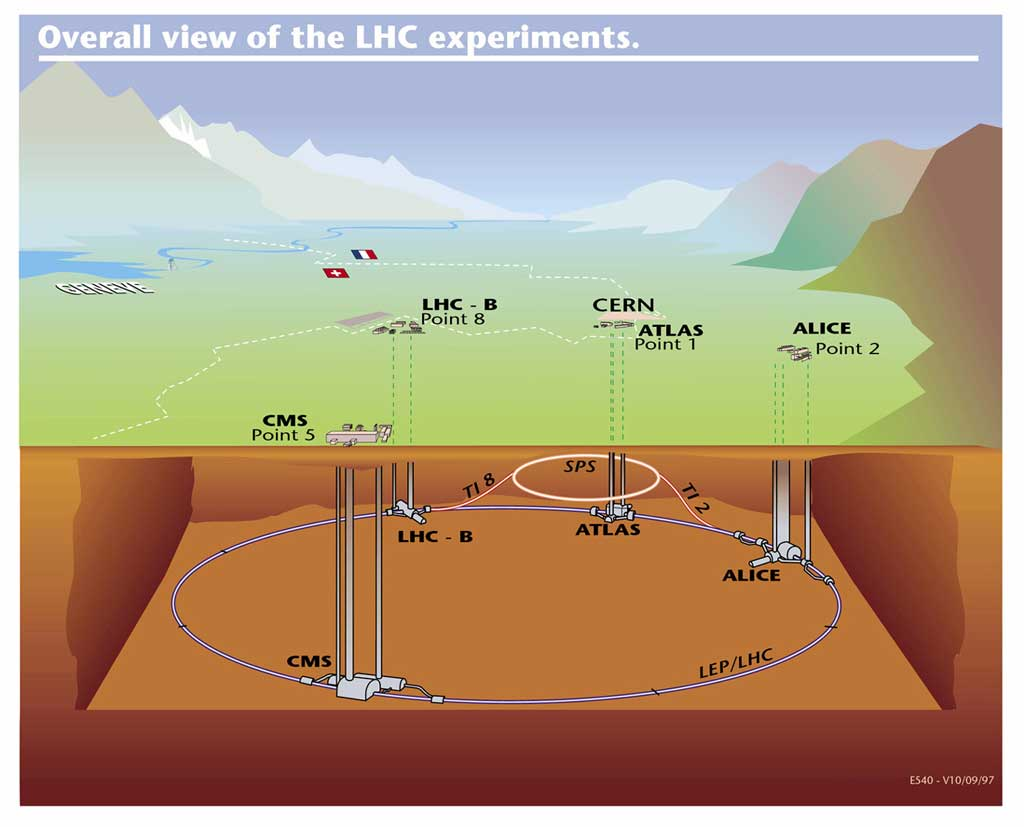
\includegraphics[width=\largefigwidth]{plots/detector/lhc_layout_sch.jpg}
  \caption{The layout of the LHC accelerator chain, showing the position of the four main detectors.??REFERENCE}
  \label{fig:lhclayout}
\end{figure}

When studying a physical process occuring in particle collisions it is important to know how many times it will occur, this can be expressed as:
\begin{equation}
  N = \mathcal{L}\sigma,
\end{equation}
where $\mathcal{L}$, the integrated luminosity, depends only on the parameters of the collisions, and the cross-section depends only on the process. In order to observe rare (i.e. low cross-section) processes it is, therefore, necessary to use very high luminosity datasets. The integrated luminosity is obtained by integrating the instantaneous luminosity over time, so large luminosities can be obtained either by running the accelerator for a long time, or by operating at high instantaneous luminosity. For collisions at the LHC the instantaneous luminosity is given by:
\begin{equation}
  \mathcal{L}=\frac{k_{b}N_{b}^{2}f_{rev}\gamma}{4\pi\epsilon_{n}\beta}, \cite{Benedikt:823808}
\end{equation}
where $k_{b}$ is the number of bunches per beam, $N_{b}$ the number of protons per bunch, $f_{rev}$ the revolution frequency, $\epsilon_{n}$ the normalised transverse beam emittance, $\beta^{*}$ the beta-function at the interaction point and $\gamma$ the Lorentz factor. The design instantaneous luminosity of the LHC is $10^{34}\,\cm^{-2}\rm{s}^{-1}$ with 25ns bunch spacing.

The LHC started physics runs in 2010, during which it operated at a centre of mass energy of 7 \TeV~ and delivered an integrated luminosity of 44.2 \invpb ~to CMS. In 2011 the LHC also operated at 7 \TeV~ and delivered 6.1\invfb to CMS. The centre of mass energy was increased to 8 \TeV~ in 2012 and 23.3\invfb~of data were delivered to CMS. A summary of the luminosity delivered to CMS during the three runs can be seen in \FigureRef{fig:lumisummary}  %??Design and actual luminosity so far 
%??Discuss operation at energies

\begin{figure}
  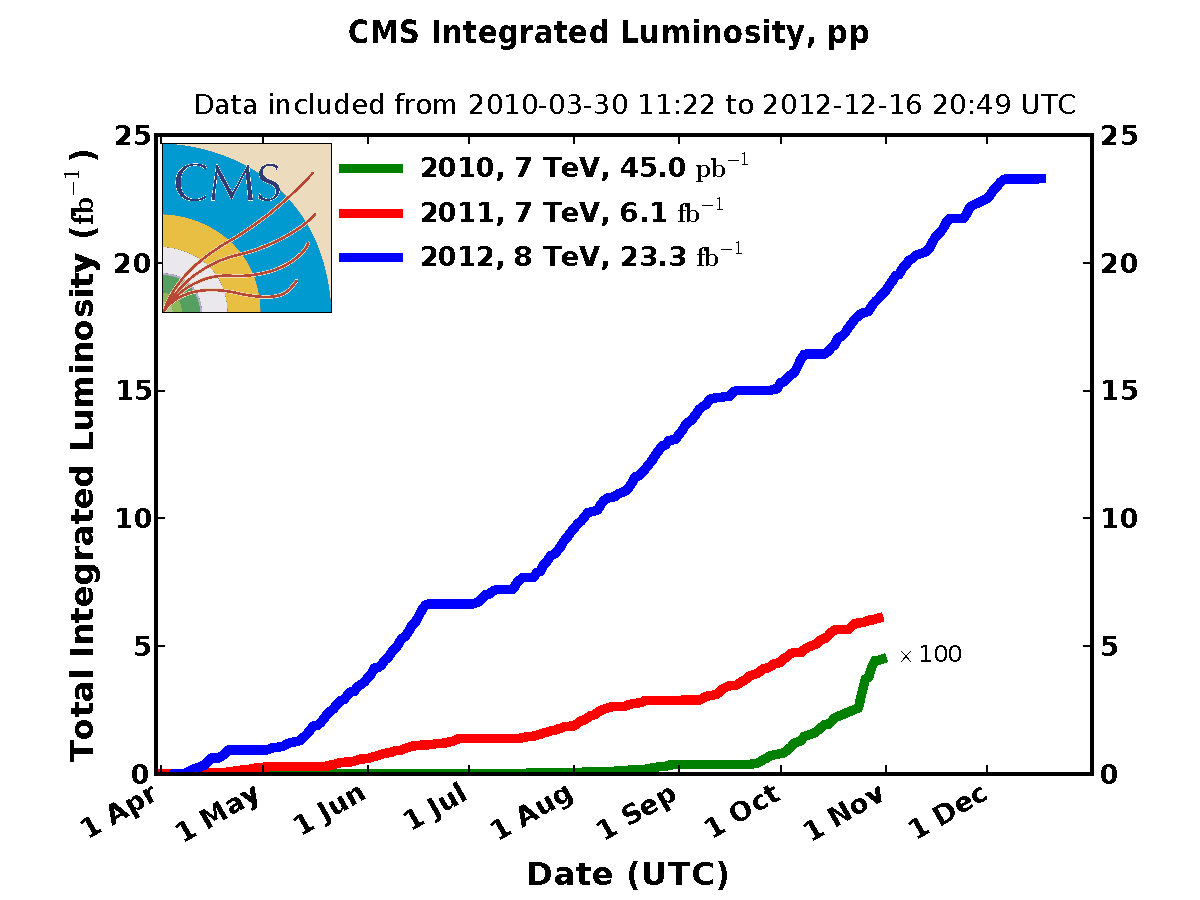
\includegraphics[width=1.2\largefigwidth]{plots/detector/int_lumi_cumulative_pp_2.pdf}
  \caption{A summary of the luminosity delivered to CMS during Run 1 of the LHC.??REFERENCE}
  \label{fig:lumisummary}
\end{figure}

The cross-section for several processes is shown in \FigureRef{fig:xs} and it can be seen that the cross-section for VBF Higgs production is approximately 1 pb. %?? implications for how many events in run 1 and backgrounds

%??Discuss pileup
%??Define an event

\section{The \CMS experiment}
\label{sec:CMSInDetail}
%??Introduction - describe hermetic onion shell concept and introduce subsystems
%??Coordinate system

\begin{figure}
  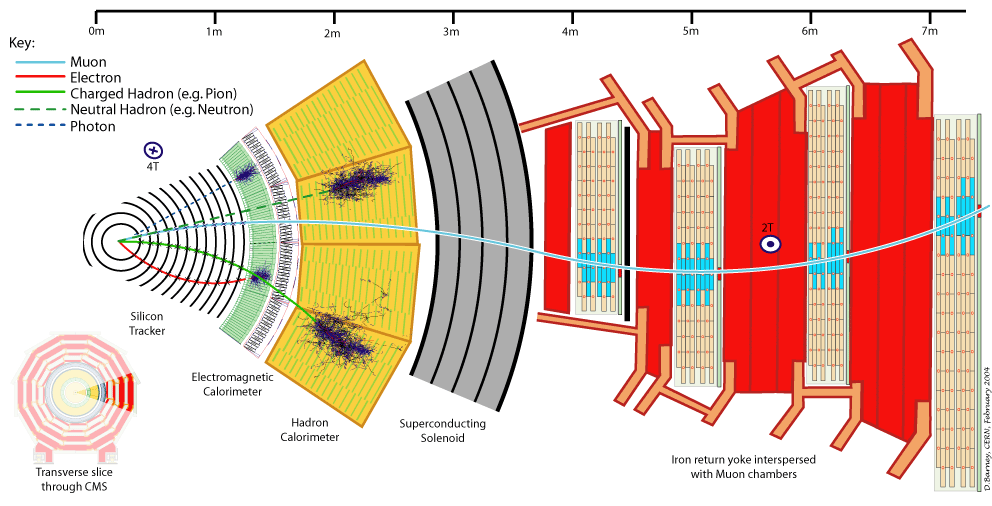
\includegraphics[width=1.2\largefigwidth]{plots/detector/CMS_Slice.png}
  \caption{A schematic cross-section of the CMS experiment showing the path taken by several types of particles.??REFERENCE}
  \label{fig:cmsschematic}
\end{figure}

\subsection{Tracker}
\label{sec:tracker}
%??Describe Tracker

\subsection{Electromagnetic calorimeter}
\label{sec:ECAL}
%??Describe ECAL

\subsection{Hadronic calorimeter}
\label{sec:HCAL}
%??Describe HCAL

\subsection{Muon system}
%??Describe muon system


\subsection{Trigger system}
\label{sec:triggers}
%??Describe trigger system

